\chapter{Background}
\label{ch:bg}
In this chapter, we discuss background information and related work for Facet Web Search, an extension of faceted search in the open-domain web setting. Faceted search is a heavily interdisciplinary area, where different aspects of information retrieval, knowledge representation, human computer interaction must be considered all together. Therefore, we first describe related topics in these areas as a background for faceted search/Faceted Web Search. Then, we describe faceted search, Faceted Web Search and previous research on these topics. After that, we discuss related approaches that aim to achieve the same goals as our work. We defer discussion of some related work to later chapters where the context makes it more appropriate.

\section{Direct Search and Navigational Search}
Faceted search combines two search paradigms, direct search and navigational search. \textbf{Navigational search} (sometimes also called \concept{directory navigation}) uses a hierarchy structure to enable users to browse the information space by iteratively narrowing the scope of their quest in a predetermined order, as exemplified by Yahoo! Directory\footnote{http://en.wikipedia.org/wiki/Yahoo!\_Directory} and DMOZ\footnote{http://www.dmoz.org/}. Navigational search provides a guided search interface, and supports abstractions that are easily understood by users. However, the strict ordering imposed by the hierarchy structure can be too rigid, especially for large and heterogeneous corpora~\cite{snow2006semantic,tunkelang2009faceted,sacco2009dynamic}. The rapid decline of Yahoo! Directory as a primary web search engine provides pragmatic evidence.

\textbf{Direct search} instead allows users to specify their own queries as input, and is the dominant paradigm in the field of information retrieval. The queries are often keywords in web search scenarios, and thus, sometimes direct search is also called \concept{keyword search}. Direct search resorts to search systems for understanding search intents behind user queries, and returns search results that could best address the search intents. This approach has been made enormously popular by web search engines, such as Google\footnote{http://www.google.com}. However, in the basic search interface, users have to formulate their queries with no or limited assistance, and no exploration capability since results are presented as a flat list with no systematic organization. Faceted search aims to solve this problem, which is described later in Section~\ref{sec:background-fs}. We also discuss other recent advances for addressing this problem in Section~\ref{sec:bg-others}.

\section{Taxonomy and Faceted Taxonomy}
There are two types of information representation (or knowledge representation) related to this work, taxonomies and faceted taxonomies.

The word \concept{taxonomy} was originally referred to the classification of biological organisms. Its history dates back to more than two millennia ago. At that time, the Greek philosopher Aristotle first classified all living things into a hierarchical classification system, a taxonomy~\cite{tunkelang2009faceted}. The taxonomy classifies living things by dividing them into two groups, plants and animals; further dividing animals into those ``red blood'' and ``no red blood''; those with no red blood into ``hard bodies'' and ``soft bodies''; and so forth (Figure~\ref{fig:bg-aristotle}).
\begin{figure}[ht!]
\centering
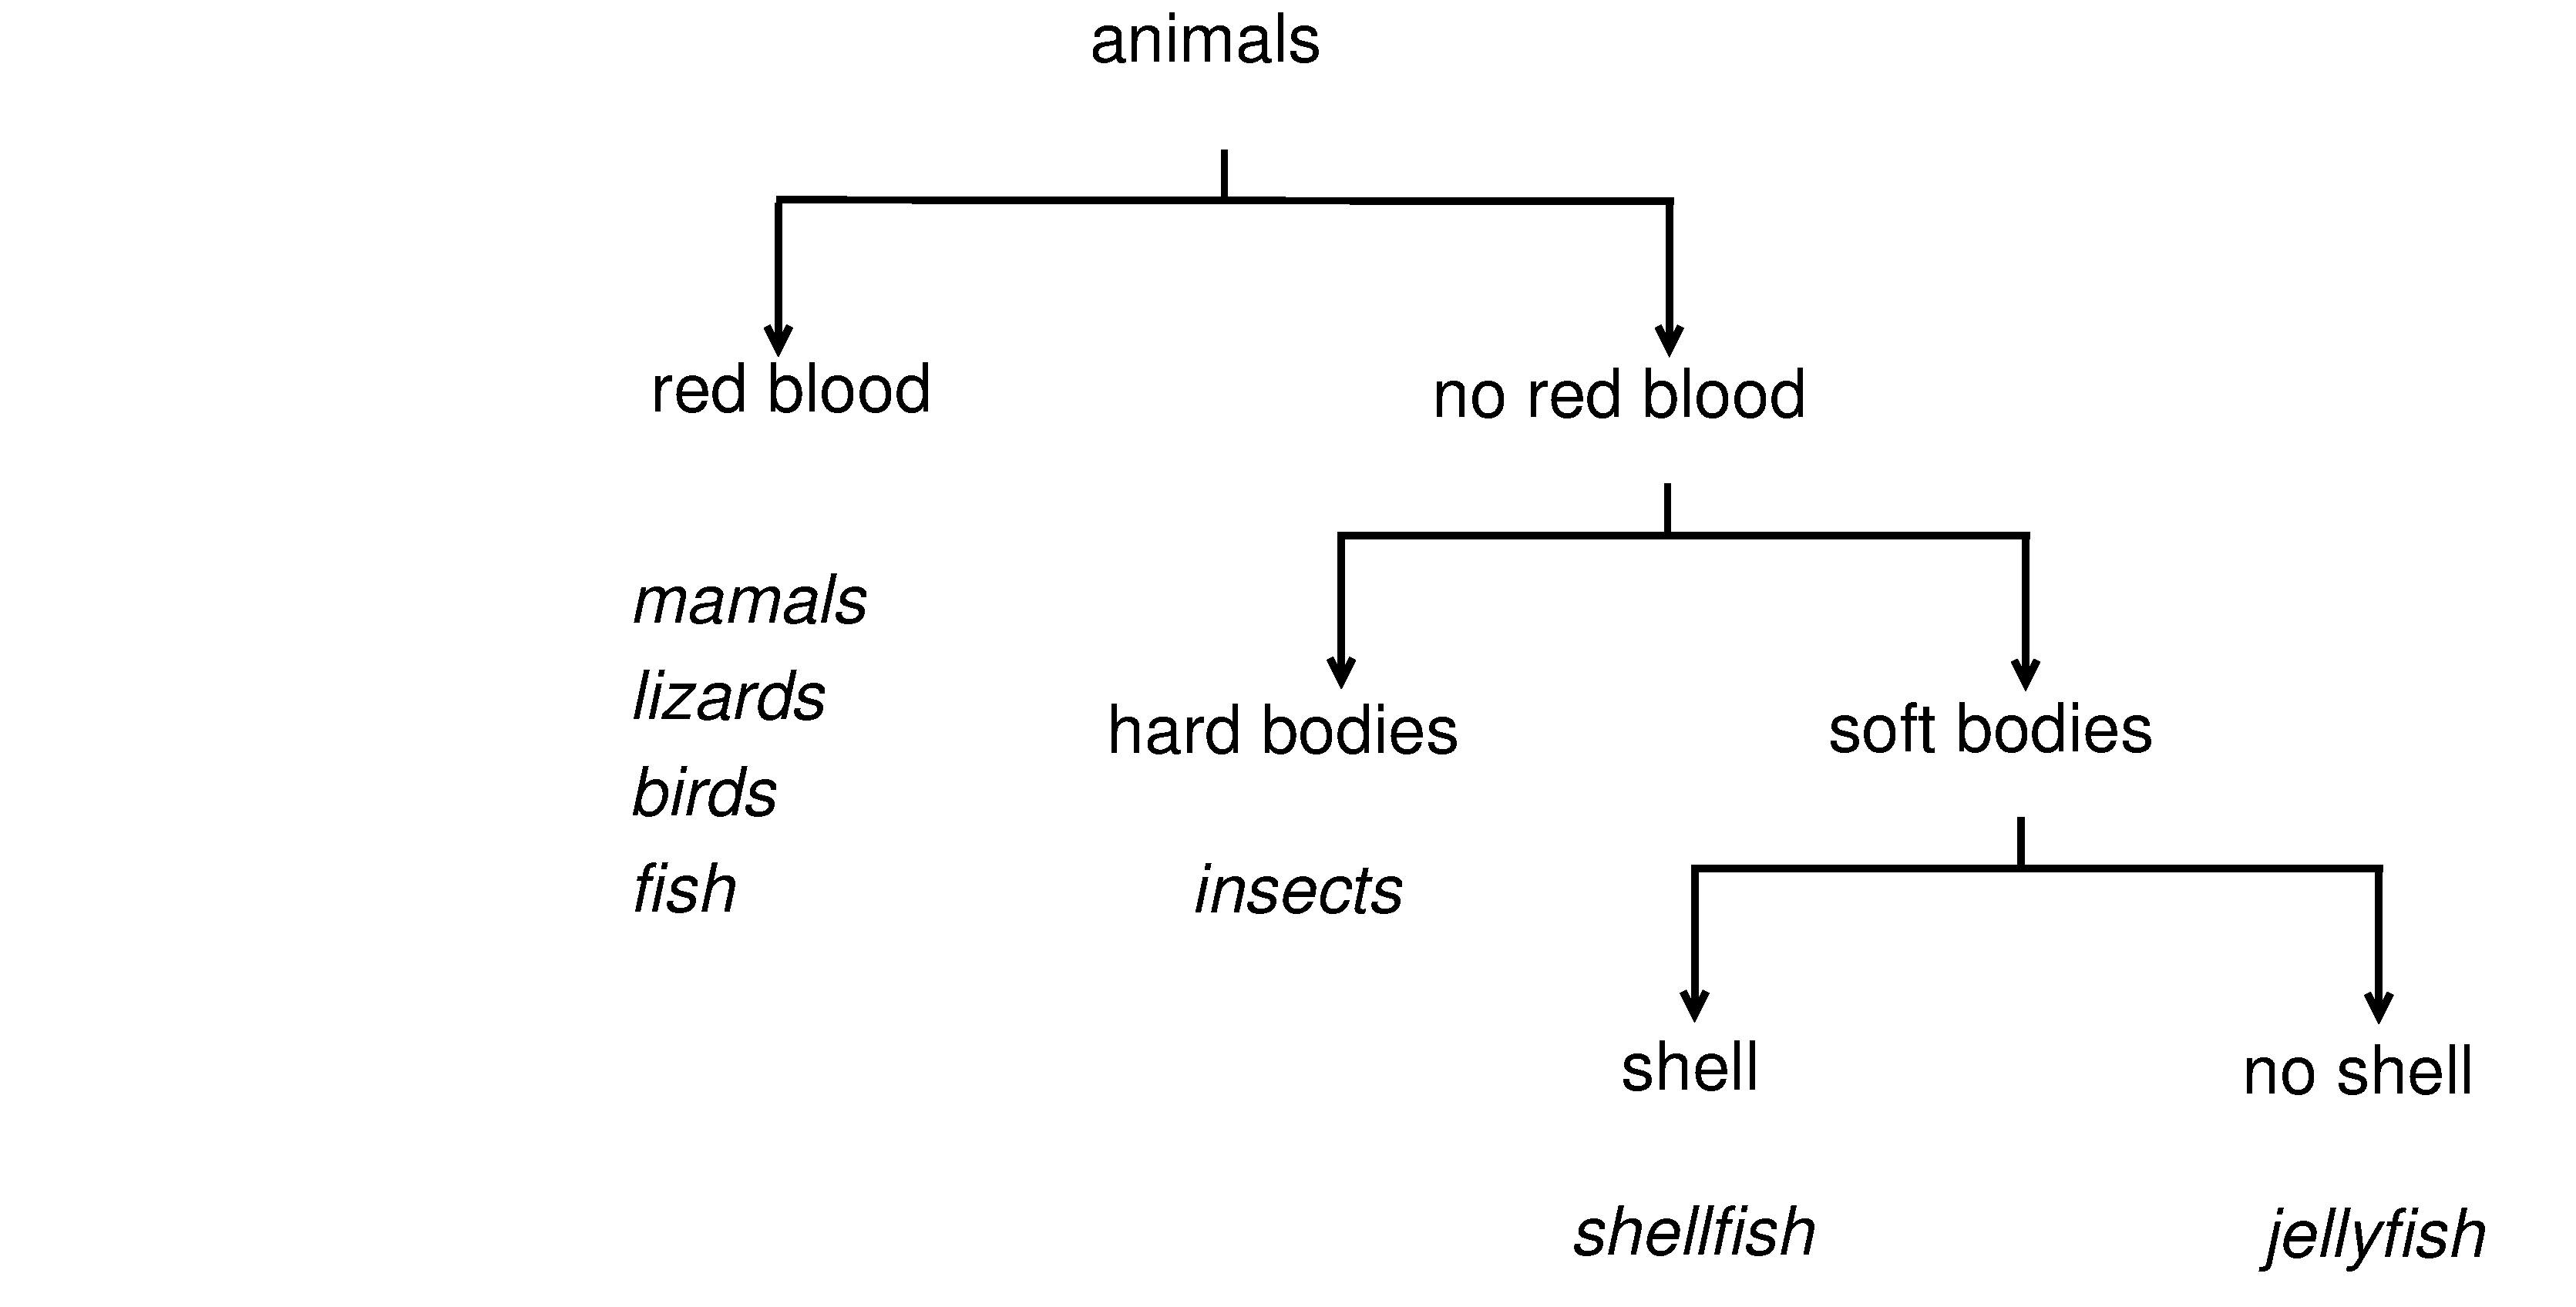
\includegraphics[width=0.95\columnwidth]{drawing/aristotle.eps}
\caption{A subset of Aristotle's knowledge taxonomy~\cite{tunkelang2009faceted}}
\label{fig:bg-aristotle}
\end{figure}

Today, the word \concept{taxonomy} refers more generally to any hierarchical classification schema. \citet{tunkelang2009faceted} described a taxonomy as an organization of things or abstractions into a hierarchy or tree structure. Similarly, \citet{sacco2009dynamic} describe a taxonomy as a concept hierarchy going from the most general to the most specific concepts, into which information objects can be classified. Using the Aristotle's taxonomy as an example, we can see that concepts or abstractions of animals are organized in a tree. The root node \concept{animals} corresponds to the set of all animals. Its children represent the top-level divisions of the animals, one representing \concept{red blood} animals and one representing \concept{no red blood} animals. Their children correspond to the subdivisions of those animals; and so forth. Information objects are classified directly into concepts in the tree. For example, the object \concept{jellyfish} is classified to the concept \concept{no shell} and the object \concept{insects} is classified to the concept \concept{hard bodies}. 

To provide a more clear definition for a taxonomy, we synthesize its previous definitions and formulations~\cite{sacco2009dynamic, tzitzikas2005compound}, and define a taxonomy as follows:
\begin{definition}
A \textbf{taxonomy} is a tree of concepts with all concepts subsuming their descendant concepts.
\end{definition}
Next we explain the terminology used in this definition. First, informally, a \textbf{tree} (, like a real but upside-down tree,) has one single root node at the top, leaf nodes at the bottom, and branches connecting each nonleaf parent node to its children. \todo{ref a formal definition of tree} Figure~\ref{fig:bg-aristotle} shows an example of tree. The root node is \concept{animals}, and the parent nodes have edges pointing to their children. \textbf{Descendants} of a node $A$ are nodes under $A$'s branch. For example, Descendants of \concept{no red blood} include \concept{hard bodies}, \concept{soft bodies}, \concept{shell} and \concept{no shell}. A tree of concepts are simply a tree using concepts as nodes.

Second, a \textbf{concept} in a taxonomy is an abstraction which identifies all the information objects classified under it (including the information objects that are classified to its descendants in the concept tree). For example, in Figure~\ref{fig:bg-aristotle}, the concept \concept{no red blood} identifies all ``no-red-blood'' animals in the taxonomy, including \concept{inserts}, \concept{shellfish}, \concept{jellyfish} classified to its descendants. More formally, a \textbf{concept} $C$ can be defined as a set of information objects $C=\{d\}$. However, before being materialized with information objects, a concept is just an abstraction for a set of potential information objects. Also, concepts are often presented by their textual labels to convey the concept meaning to users.

Last, in the definition, the concept tree is constrained by having concepts in the tree subsumes all its descendant concepts. A concept $A$ is \textbf{subsumed} by a concept $B$ ($A \preccurlyeq B$) if the set of information objects classified under $A$ is intensionally constrained to be equal to or a subset of the set of objects classified under $B$: $A \subseteq B$. For example, in Figure~\ref{fig:bg-aristotle}, we can say that the concept \concept{shell} is subsumed by the concept \concept{no red blood}, because every animals classified under \concept{shell} is also classified under \concept{no red blood}. This definition of subsumption indicates a reflexive and transitive binary relation over concepts. It is very general, and thus can model many different reflexive and transitive binary semantic relations, such as IS-A and PART-OF. For example, the subsumption relation \concept{shell} $\preccurlyeq$ \concept{no red bold} indicates a ``shell'' animal is a ``no-red-blood'' animal. For PART-OF relations, an example is a taxonomy of United States locations in which the concept \concept{USA} has a child node \concept{MA}, and the concept \concept{MA} has a child node \concept{Amherst}. Thus, we have \concept{MA} $\preccurlyeq$ \concept{USA},  \concept{Amherst} $\preccurlyeq$ \concept{MA} and \concept{Amherst} $\preccurlyeq$ \concept{USA} (from the transitive property). Here the subsumption relations between these locations model PART-OF relations (\eg, \concept{MA} is a part of \concept{USA}).



%Based on the definitions of concepts and subsumption, a taxonomy can be defined as a tree of concepts with the concepts subsuming all their descendant concepts, or more formally:
%\begin{definition}
%A \textbf{taxonomy} is a tree $(\mathcal{C}, E)$, where $\mathcal{C}=\{C\}$ is a set of concepts and the nodes in the tree. $E$ is the set of edges in the tree. For any $C\in\mathcal{C}$ and any $C'$ in $Descendant_E(C)$, $C' \preccurlyeq C$, where $Descendant_E(C)$ is the set of all descendant nodes of $C$ in the tree, and $\preccurlyeq$ is the subsumption relation.
%\end{definition} 
%\citet{tzitzikas2005compound} provided a formal definition for a taxonomy:
%\begin{definition}
% A \textbf{taxonomy} is a pair $(\mathcal{C}, \preccurlyeq)$, where $\mathcal{C}=\{C\}$ is a set of concepts, and $\preccurlyeq$ is a subsumption relation over $\mathcal{C}$.
%\end{definition}
%In applications, a taxonomy is organization of concepts into a hierarchy or tree structure. 
%Directed acyclic graph taxonomies modeling multiple inheritance are supported.
%For example, in the Aristotle's taxonomy, \concept{red blood} is a concept that has objects \concept{mamals}, \concept{lizards}, \concept{birds}, \concept{}



Navigational search as described above is based on taxonomies. So we have seen two examples of taxonomies, Yahoo! Directory and the Open Directory Project, in which webpages are classified into the hierarchies. 

In the context of navigational search, taxonomy enables efficient navigation in the information space. Users start from the root node and iteratively discriminate among children, in order to find the appropriate one. Each time a node is selected for expansion, the total number of objects to be considered is reduced because the objects classified under discarded concepts need not be considered. Thus, users iteratively reduce the number of information objects to be manually inspected~\cite{sacco2009dynamic}.

The key property of a taxonomy is that, for every information object or set of objects that corresponds to a node, there is precisely one unique path to it from the root node. Thus, a taxonomy imposes a strict logical ordering on the information that it represents~\cite{tunkelang2009faceted}. For example, \concept{cancer} can be classified in a taxonomy with a unique path  \concept{disease}$\rightarrow$\concept{structural disease}$\rightarrow$\concept{tumor}$\rightarrow$\concept{cancer}. However, this strict ordering of a taxonomy can be too rigid when dealing with compound information objects. For example, should \concept{treatment of cancer} be a child of \concept{treatment} or of \concept{cancer}? This strict ordering constraint limits expressibility and extensibility of taxonomies and navigational search systems build on them.

Faceted search is based on another type of information representation, called faceted taxonomy, which is sometimes also called multi-dimensional  taxonomy~\cite{sacco2009dynamic} or faceted classification~\cite{tunkelang2009faceted}. A \textbf{faceted taxonomy} is a set of independent taxonomies where each one organizes information objects from a different (preferably orthogonal) point of view, or equivalently based on a different dimension of the multi-dimensional information space. For example, in \textit{Classification, Coding, and Machinery for Search}, \citet{ranganathan1950classification} describe a library system based on a faceted taxonomy for organizing books, with four independent taxonomies mentioned -- the taxonomy \concept{Medicine}, \concept{Disease}, \concept{Treatment} and \concept{Mathematical study}. The four taxonomies each represents one dimension of the multi-dimensional information space for the books. \todo{better example for faceted taxonomy}


The advantage of using multiple independent taxonomies is that they can be combined to describe compound information objects. In Ranganathan's example, the four taxonomies are combined to expresses the topic \concept{statistical study of the treatment of cancer of the soft palate by radium}, as follows. 
\begin{itemize}
 \item Medicine $\rightarrow$ Digestive system $\rightarrow$ Mouth $\rightarrow$ Palate $\rightarrow$ Soft palate
\item Disease $\rightarrow$ Structural disease $\rightarrow$ Tumor $\rightarrow$ Cancer
\item Treatment $\rightarrow$ Treatment by chemical substances $\rightarrow$ Treatment by a chemical element  $\rightarrow$ Treatment by a group 2 chemical element $\rightarrow$ Treatment by radium
\item Mathematical study $\rightarrow$ Algebraical study $\rightarrow$ Statistical study
\end{itemize}
The foci (\concept{Soft palate}, \concept{Cancer}, \concept{Treatment by radium} and \concept{Statistical study}) in each of the taxonomies are combined to express the compound topic, which is difficult in a single hierarchical taxonomy. Combining these independent taxonomies, faceted taxonomies offer expressive power and flexibility beyond single taxonomy used in navigational search. 

%From the example, we can also see that faceted taxonomy enables navigation over , which is called \textbf{faceted navigation}.
Navigation based on a faceted taxonomy is called \textbf{faceted navigation}. In faceted navigation, users can use multiple taxonomies to navigate or explore a multi-dimensional information space. They can narrow the search space by iteratively select child nodes in each of taxonomies. Then the selections on the taxonomy are combined to restrict the matched information objects, as has illustrated in Ranganathan's example and the computer monitor example (Figure~\ref{fig:intro-amazon}).
\todo{add an example}
\todo{relationships to scatter/gather, clustering}

Faceted navigation is also related to search results clustering or organization, which is discussed in Section~\ref{sec:bg-others}

%pose a challenge for the hierarchical organization of single taxonomies.
\section{Facets}
``Facet'' is a key concept in faceted search. The term \concept{facet} means ``little face'' and is often used to describe one side of a many-sided object, especially a cut gemstone~\cite{teevan2008challenges}. In information science literature, \concept{facet} is a overloaded term. The term has been used to refer both to the entire independent taxonomies in a faceted taxonomy, and to the part of independent taxonomies that are shown to users (as in most of our discussion). In many cases the taxonomies are often shown as shallow or two-level trees. In the computer monitor example (Figure~\ref{fig:intro-amazon}), the facets are two-level (\eg, parent node \concept{Brand} with child nodes \concept{Dell}, \concept{ViewSonic}, \concept{HP}, \concept{Acer}). When there are only two levels in a facet, we can call the parent node (or more precisely, its presentation term) a \textbf{facet label} (\eg, \concept{brand}), and the child nodes \textbf{facet terms} (\eg, \concept{Dell}, \concept{ViewSonic}). It is easy to 
see that in a two-level facet, facet terms belong to the same semantic class (\ie, the semantic class represented by their parent node). Sometimes, a facet label can be missing or omitted, which results in a one-level facet. So a one-level facet consists of only facet terms (\eg, \{\concept{Dell}, \concept{ViewSonic}, \concept{HP}, ...\}) with no facet labels. This work focuses on studying one-level facets for Faceted Web Search as a start, and leaves the extension of two-level facets to future work.

\todo{exploratory search}

\section{Faceted Search}
\label{sec:background-fs}
\textbf{Faceted Search} combines direct search with faceted navigation, which enables users to navigate a multi-dimensional information space. We have provided an example in Figure~\ref{fig:intro-amazon}. In the example, a user searches with the query \concept{computer monitor} in an e-commercial site, and the site provides the two-level facet \concept{brand}, \concept{display technology} and \concept{condition} for users to select and filter the search results.

Compared with direct search, faceted search provides additional search assistance for users through facets. Facets can assist users in clarifying their search intent and refining the search results (\eg, select \concept{new} in facet \concept{condition} to find only computer monitors in new conditions). Facets also summarize the search space succinctly, and provides exploration suggestions organized in a systematic way (\eg, the listed facet \concept{brand}, \concept{display technology}, \concept{condition} give users an overview of the returned results, and provides them with the key factors they may need to consider when searching for a computer monitor). This exploration capability is especially important in exploratory search tasks, or when users are not exactly clear about what they are looking for~\cite{kules2009exploratory,sacco2009dynamic}.

Compared with navigational search, faceted search is based on a faceted taxonomy that enables faceted navigation, which, as outlined above, is especially useful for navigating a multi-faceted information space. In navigational search, the strict ordering imposed by a taxonomy is too rigid when dealing with compound information objects in the multi-faceted information space. Instead, in faceted search, users can combine facets to express complex information need (\eg, \concept{statistical study of the treatment of cancer of the soft palate by radium} in  Ranganathan's example).

The principle of faceted taxonomy used in faceted search is widely applicable. In research literature, there are faceted search systems developed for a wide range of domains, including images~\cite{yee2003faceted}, movies~\cite{koren2008personalized}, desktop content~\cite{cutrell2006fast}, audio content~\cite{diao2010faceted}, houses~\cite{shneiderman1994dynamic}. \todo{can include more}For commercial applications, faceted search have been adopted by vendors such as Endeca\footnote{http://en.wikipedia.org/wiki/Endeca} and IBM\footnote{https://en.wikipedia.org/wiki/IBM}, and it is now the dominant search paradigm used in e-commercial sites, such as Amazon\footnote{http://www.amazon.com/} and eBay\footnote{http://www.ebay.com/}.

\section{Faceted Web Search}
Despite the success of faceted search in vertical applications, there is limited work in exploring \textbf{Faceted Web Search}, an extension of faceted search to the open-domain web~\cite{kong2014extending}. In the open-domain web setting, the corpus or the collection of information objects considered is the entire web, not restricted to any given domains as in the vertical applications. But as conventional faceted search, Faceted Web Search should also provide facets to assist users in the same principle. We have shown an example of Faceted Web Search in Figure~\ref{fig:fws-example}, in which the user searches with the web query \concept{baggage allowance}, and the Faceted Web Search system provides a list of facets including  as a facet for different airlines, \{\concept{Delta}, \concept{JetBlue}, \concept{AA}, ...\}, a facet for different flight types, \{\concept{domestic}, \concept{international}\}, and a facet for different classes, \{\concept{first}, \concept{business}, \concept{economy}\}. The user 
can then select some facet terms in the facets to refine or explore the search results.

The challenge of Faceted Web Search stems from the facet that the web is very large and heterogeneous, as discussed by \citet{teevan2008challenges}. From a system perspective, because the web is very large, it is infeasible to build a complete faceted taxonomy for the entire web manually. And because the web is heterogeneous, it is also difficult to develop automatic methods for generating facets for the entire web. From a user perspective, users conduct a wide range of search tasks on this large and heterogeneous corpus. Queries applied to the web are varied in intent, which makes it difficult to predefine a set of facets for all the queries. Next, we describe existing work for generating facets in faceted search.

%To cope with these challenges, our work extracts facets from the search results of a given query, which makes the problem much easier.
\section{Facet Generation}
In conventional faceted search, facets are typical generated manually or can be derived directly from the structured data~\cite{basu2008minimum,yee2003faceted,dash2008dynamic,ben2008beyond}. For example, in e-commerce sites such as Amazon~\footnote{http://wwww.amazon.com}, products are stored as structured data with manually created schema. Each product is attached with related attributes such as \concept{brand}, \concept{price}, \concept{condition}, etc. These attributes can be directly used as facets for these products. \citet{basu2008minimum} also used 19 attributes (\eg, \concept{actor}, \concept{genre}) as facets for a movie databases, and used 43 attributes (\eg, \concept{made}, \concept{model}, \concept{mileage}) as facets for a car database. As discussed before, since the web is large and heterogeneous, it is infeasible to generated facets or build such databases for it manually.

Previous work that automatically generates facets (or a single taxonomy) is typical based on some existing thesaurus or knowledge bases, such as WordNet~\cite{stoica2007automating,dakka2005automatic,dakka2008automatic,latha2010afgf} and Wikipedia~\cite{dakka2008automatic,li2010facetedpedia,kohlschutter2006using}. The idea is to leverage the hierarchical structures already built in these resources. For example, \citet{stoica2007automating} created taxonomies for a corpus consists of 13,000 recipes using the hierarchical structure base on the hypernym (IS-A) relations in the WordNet~\cite{fellbaum1998wordnet}. They first selected a subset of terms that are intended to best reflect the topics in the documents. Then they created taxonomies using the selected terms by mapping into the WordNet, and leveraging the IS-A relations in the WordNet to build hierarchical structure of these selected terms. \citet{li2010facetedpedia} build a faceted search system for Wikipedia by inducing taxonomies from the existing 
category hierarchy and link structures in it. \citet{dakka2008automatic} generated facets for news corpora by first selected keywords in the news articles (as facet terms), and then used hypernyms in WordNet as well as link structures in Wikipedia to assign facet labels for the selected terms. However, using thesaurus with the knowledge bases alone also restricts the extensibility of these facet generation methods to the general and open-domain settings, thus most of the work applied the methods only in a domain-specific setting or only for copora that have direct associations in the knowledge bases. Our work instead is for a more general setting, targeting facet generation for the entire web.
\todo{can be more extensive}
%Previous work on faceted search has studied automatic facet generation ~\cite{dakka2008automatic,li2010facetedpedia,stoica2007automating,oren2006extending,kohlschutter2006using,latha2010afgf} and facet recommendation for a query~\cite{dash2008dynamic,koren2008personalized}. Most of the work is based on existing facet metadata or taxonomies, and extending faceted search to the general web is still an unsolved problem. The challenges stem from the large and heterogeneous nature of the web~\cite{teevan2008challenges}: because the web is very large, it is difficult to assign quality facets to every document in the collection and to retrieve the full set of search results and their associated facets at query time; and because the web is heterogeneous, it is difficult to apply the same facets to every search result or every query.
%Different from previous work which generates facets for a entire corpus~\cite{stoica2007automating,dakka2008automatic}, some recent work~\cite{dou2011finding,kong2013extracting} extracts facets for only a query.

\todo{facet recommendation}
\section{Faceted Search User Interface}
User interface is an important factor for faceted search and attracts lots of research attention. The goal is to design a faceted search interface that help users to make effective uses of facets -- an user interface that supports flexible faceted navigation with directed search and at all times retaining a feeling of control and understanding. From a more general perspective, for users to make effective use of search refinement options, the refinements must offer users what \citet{pirolli2000effect} call \textbf{information scent}: cues that indicate to users the value, cost of accessing the refinement options. In the context of faceted search, it is thus important that users are provided with some indicators about the effect for accessing each facets or facet terms. This is typically accomplished by displaying facet terms with the counts of matched search results for each terms. For example, in Figure~\ref{fig:intro-amazon}, the facet \concept{display technology} and \concept{condition} are shown together 
with the numbers of matched computer monitors for each facet terms (\eg, 25,581 for \concept{new} condition, and 2,959 for \concept{used} condition). \citet{ben2008beyond} investigated more sophisticated method that returned not only counts of the matched search results for facets, but also richer aggregations that could support more effective decision making. For example, when shopping for books and looking to refine the search by facet \concept{author}, it might make more sense to drill down to the author who wrote the most bestsellers, instead of focusing on the author who wrote the most books. So they showed not only the counts of books matched for each authors, but also the numbers of best sellers for them.

The Flamenco project led by Marti Hearst was the most visible research project focusing on faceted search, and especially the user interface aspect of it. The goals of the Flamenco project were to investigate how to assist navigation and browsing of information collections via the use of facets or other hierarchical taxonomies. They addressed questions such as how to allow the user to navigate in several hierarchies simultaneously, how to show facets and matched search results, how to display the query as it is built up, how to present the query previews, and so on. \citet{hearst2006design} provided a nice summary of the best practices in user interface design for faceted search.

\section{Faceted Search Evaluation}
Compared to the mature evaluation methodology for information retrieval systems, evaluation of faceted search is still nascent~\cite{wilson2009bridging,tunkelang2009faceted}. Most evaluations for faceted search are based on user studies and focus on the user interface aspect~\cite{burke1996knowledge,english2002hierarchical,hearst2006design,yee2003faceted,hearst2008uis,kules2009exploratory}.
For example, via usability studies, \citet{yee2003faceted} show that when incorporated into a properly-designed user interface, hierarchical facets provides a flexible, intuitive way to explore a large collection of items that enhances feelings of discovery without inducing a feeling of being lost.
The evaluations for facet generation are also typically based on user studies~\cite{li2010facetedpedia,stoica2007automating}. For example, \citet{li2010facetedpedia} conducted user studies to evaluate the effectiveness of generated facets for Wikipedia. They showed facets generated by different methods to the human subjects, then the subjects were administered a questionnaire asking questions, such as \concept{which interface is better than the other?}, \concept{what is your rating about usefulness of the interface}. The questionnaire results were aggregated for evaluating generated facets. While user studies provide a direct evaluation for faceted search, they are typically expensive, and more importantly difficult to extend for evaluating new systems or methods. We instead design evaluation methods for faceted search that are much easier to be reused for evaluating new systems.
 
%Most evaluations for facet generation/recommendation are either based on comparison between system generated and human created facets~\cite{dakka2008automatic,dou2011finding} or user studies~\cite{dash2008dynamic,li2010facetedpedia,stoica2007automating}. However, the former may not exactly reflect the utility of assisting users' search tasks, and the latter is expensive to extend for evaluating new systems. In a spirit similar to ours, some work~\cite{schuth2011evaluation,zhang2010interactive,koren2008personalized} also evaluates facets by their utility in re-ranking documents for users. The differences are their evaluation methods do not capture the time cost for users as explicitly as we do, and their experiments are based on corpora with human created facet metadata. Other evaluations~\cite{burke1996knowledge,english2002hierarchical,hearst2006design,hearst2008uis,kules2009exploratory} for faceted search are mostly done from a user interface perspective, which is beyond the scope of this proposal.

\section{Other Related Techniques}
\label{sec:bg-others}
There are a number of techniques developed to achieve similar goals as faceted search or faceted web search. In this section, we discuss query subtopic mining, semantic class extraction, search result diversification and search result clustering/organization.
\subsection{Query Subtopic Mining}
To address multi-faceted queries, much previous work studied mining query subtopics (or aspects). A query subtopic is often defined as a distinct information need relevant to the original query. It can be represented as a set of terms that together describe the distinct information need~\cite{wang2009mining,wu2011identifying, dang2011inferring} or as a single keyword that succinctly describes the topic~\cite{song2011overview}. 

Different resources have been used for mining query subtopics. \citet{wang2007learn} and \citet{hu2012mining} used related queries from search logs as candidates, and clustered them into query subtopics. \citet{wang2007learn}, for example, used snippets of a query's clicked web documents to enrich the query representation, and then cluster related past queries into query subtopics.
Due to data sparsity for instance-level query subtopics, some work~\cite{wang2009mining,xue2011topic,wu2011identifying,yin2010building} mined generic query subtopics, which are query subtopics for a generic class of queries. For example, \citet{yin2010building} built taxonomies of query subtopics for categories of name entity queries using search logs. \citet{wu2011identifying} also worked on identifying query aspects for named entities queries. They propagated reformulation phrases for a classes of named entities queries. Other than query logs, query subtopics can also be mined from documents. For example, \citet{dang2011inferring} worked on clustering related anchor texts in ClueWeb09 corpus into query subtopics. \citet{allan2002using}, from a text corpus, extracted commonly occurring parts of speech pattern near a single-word query to find different potential specifications of the query.
\todo{top ranked documents}

Query subtopics and facets for a query are different in that the terms in a query subtopic are not restricted to be coordinate terms, or to have peer relationships. Facets for a query, however, organize terms by grouping ``sibling'' terms together. For example, \{\textit{news}, \textit{cnn}, \textit{latest news}, \textit{mars curiosity news}\} is a valid query subtopic for the query \textit{mars landing}, which describes the search intent of Mars landing news, but it is not a valid facet. Instead, a valid facet that describes Mars landing news could be \{\textit{cnn}, \textit{abc}, \textit{fox}\}, which includes different news channels.
%In a recent work~\cite{Dou:2011:FDQ:2063576.2063767}, Dou et al. developed a system to extract facets from web search results and showed the potential of doing so. However, the unsupervised method they proposed is far from optimal, and it does not improve by having human labels available. Also, to the best of our knowledge, their evaluation can be problematic in some cases, which will be discussed in Section~\ref{sec:evalmetricsall}.

\subsection{Semantic Class Extraction}
Semantic class extraction is to automatically mine semantic classes represented as their class instances from certain data corpora. For example, it may extract \textit{USA}, \textit{UK}, \textit{China} as class instances of semantic class \textit{country}. Due to the similar semantic relationships between terms inside a facet and a semantic class, semantic class extraction can be used for facet generation. Existing approaches can be roughly divided into two categories: distributional similarity and pattern-based~\cite{shi2010corpus}. The distributional similarity approach is based on the distributional hypothesis~\cite{Harris}, that terms occurring in analogous contexts tend to be similar. Different types of contexts have been studied for this problem, including syntactic context~\cite{pantel2002discovering} and lexical context~\cite{pantel2004towards,agirre2009study,pantel2009web}.
The pattern-based approach applies textual patterns~\cite{hearst1992automatic,pasca2004acquisition}, HTML patterns~\cite{shinzato2007simple} or both~\cite{zhang2009employing,shi2010corpus} to extract instances of a semantic class from some corpus.
The raw semantic class extracted can be noisy. To address this problem, \citet{zhang2009employing} used topic modeling to refine the extracted semantic classes. Their assumption is that, like documents in the conventional setting, raw semantic classes are generated by a mixture of hidden semantic classes.
In this work, we apply pattern-based semantic class extraction on the top search results to extract candidates for facet generation, and design some features based on distributional similarity for refining facet candidates.

\subsection{Search Results Diversification}
Search result diversification has been studied as a method of tackling ambiguous or multi-faceted queries while a ranked list of documents remains the primary output feature of Web search engine today~\cite{agrawal2009diversifying,clarke2008novelty,santos2010exploiting,sakai2011evaluating,dang2013term}. The purpose is to diversify the ranked list to account for different search intents or query subtopics. A weakness of search result diversification is that the query subtopics are hidden from the user, leaving him or her to guess at how the results are organized. Faceted Web Search addresses this problem by explicitly presenting different facets of a query using groups of coordinate terms for users to select.
\todo{difference}

\subsection{Search Result Clustering and Organization}
Search results clustering is a technique that tries to organize search results by grouping them into, usually labeled, clusters by query subtopics~\cite{cutting1992scatter,kaki2005findex,zamir1999grouper,carpineto2009survey}. It offers a complementary view to the flat ranked list of search results.
Most previous work has exploited different textual features extracted from the input texts and applied different clustering algorithms with them.

Instead of organizing search results in groups, there is also some work~\cite{lawrie2001finding,lawrie2003generating, nevill1999lexically} that summarizes search results or a collection of documents in a topic hierarchy. For example, previous studies~\cite{lawrie2001finding,lawrie2003generating} used a probabilistic model for creating topical hierarchies, in which a graph is constructed based on conditional probabilities of words, and the topic words are found by approximately maximizing the predictive power and coverage of the vocabulary. \todo{similar to taxonomy}


Faceted Web Search is different from these work in that it provides facets of a query, instead of directly organizing the search results. The facet interface allows users to filter/re-rank search results from multiple aspects, instead of a single taxonomic order. The utility of faceted search interface was investigated in various studies~\cite{pollitt1998key,hearst2006clustering,pratt1999knowledge,yee2003faceted,kaki2005findex,rodden2001does}, where it was shown that users engaged in exploratory tasks often prefer the faceted search interface over simple ranked result list, as well as the alternative ways of organizing retrieval results.


%\section{User Feedback}
%There is a long history of using user explicit feedback to improve retrieval performance. In relevance feedback~\cite{rocchio71relevance,salton90improvingretrieval}, documents are presented to users for judgment, after which terms are extracted from the judged relevant document, and added into the retrieval model. In the case where true relevance judgments are unavailable, top documents are assumed to be relevant, which is called pseudo relevance feedback~\cite{buckley1995automatic,abdul2004umass}. Because a document is a large text unit which can be difficult for users to judge and for the system to incorporate relevance information, previous work also studied user feedback on passages~\cite{allan1995relevance,xu1996query} and terms~\cite{koenemann1996case,tan2007term}.

%For faceted search, previous work~\cite{zhang2010interactive} studied user feedback on facets, using both boolean filtering and soft ranking models. However, the study is based on corpora with human created facet metadata, which is difficult to obtain for the general web. One other difference between our work and most other user feedback work is, facet feedback in our work is used to improve ranking with respect to the query subtopic specified by the feedback terms, instead of the query topic represented by the original query. This presents the scenario in Faceted Web Search, where users start with a less-specified query, and then use facets to help clarify and search for subtopic information.

\section{Summary}
Faceted search is the combination of directed search and faceted navigation which enables users to search and navigate through a multi-dimensional information space. Faceted navigation is based on a faceted taxonomy consists of a set of independent single taxonomies to be combined for expressing compound information needs. Faceted Web Search, the focus of this work, is the extension of faceted search to the open-domain web setting. We use the term \concept{facets} to refer the part of faceted taxonomies that are shown to users. For two-level facets, we call the parent node \concept{facet label}, and the child node \concept{facet terms}. As a start for Faceted Web Search, this work focuses on studying one-level facets, which consist of only facet terms with no facet labels.

Faceted Web Search we propose in this work is different from all the past work. It extends conventional faceted search from a fixed-domain setting to an open-domain web setting. It is different from search result diversification in that instead of hiding those query subtopics from users, it explicitly presents different facets of a query. It is also different from search results clustering or organization in that instead of directly organizing the search results, the facet interface in Faceted Web Search allows users to filter/re-rank search results from multiple aspects.

We study three main issues of Faceted Web Search that have not been explored in previous work, including facet generation, facet feedback and evaluation for Faceted Web Search. Facet generation for Faceted Web Search is different from query subtopic mining due to the different nature of query subtopics and facets. It is also different from semantic class extraction in that it targets a general web query instead of a semantic class. Facet feedback for Faceted Web Search is different from other user feedback due to their different purposes (discussed in later Section~\ref{sec:feedback-related}). Facet feedback targets at improving ranking with respect to the ``query subtopic'' specified by the feedback terms, instead of the query topic represented by the original query. Our evaluation for Faceted Web Search is also different from previous ones for faceted search in that we do not rely on expensive user studies, and thus our evaluating methods are relative cheap to extend for evaluating new systems.